\documentclass[a4paper,10pt]{article}
\usepackage[utf8]{inputenc}
\usepackage{hyperref}
\usepackage{graphicx}
\usepackage[margin=1.5 cm]{geometry}
\usepackage{helvet} 
\renewcommand{\familydefault}{\sfdefault}

\usepackage{xcolor}
\usepackage{listings}
\lstset{basicstyle=\ttfamily,
  showstringspaces=false,
  commentstyle=\color{red},
  keywordstyle=\color{blue},
  breaklines=true, % sets automatic line breaking
  postbreak=\raisebox{0ex}[0ex][0ex]{\ensuremath{\color{red}\hookrightarrow\space}},
  frame=single, % adds a frame around the code
  rulesepcolor=\color{gray}
}

\newcommand{\link}[1] {\href{#1}{#1}}
% \setlength{\parskip}{5 mm}

%opening
\title{WoWWee MiP}
\author{Arnaud RAMEY}

\begin{document}

\maketitle
\tableofcontents
\hrule
\vspace{5 mm}

\href{http://joost.damad.be/2013/08/experiments-with-bluetooth-low-energy.html}
     {joost.damad.be}
\href{https://www.safaribooksonline.com/library/view/getting-started-with/9781491900550/ch04.html}
 {safaribooksonline}
 
 \subsection{Discover all primary services}
\begin{figure}[!ht]
  \centering
  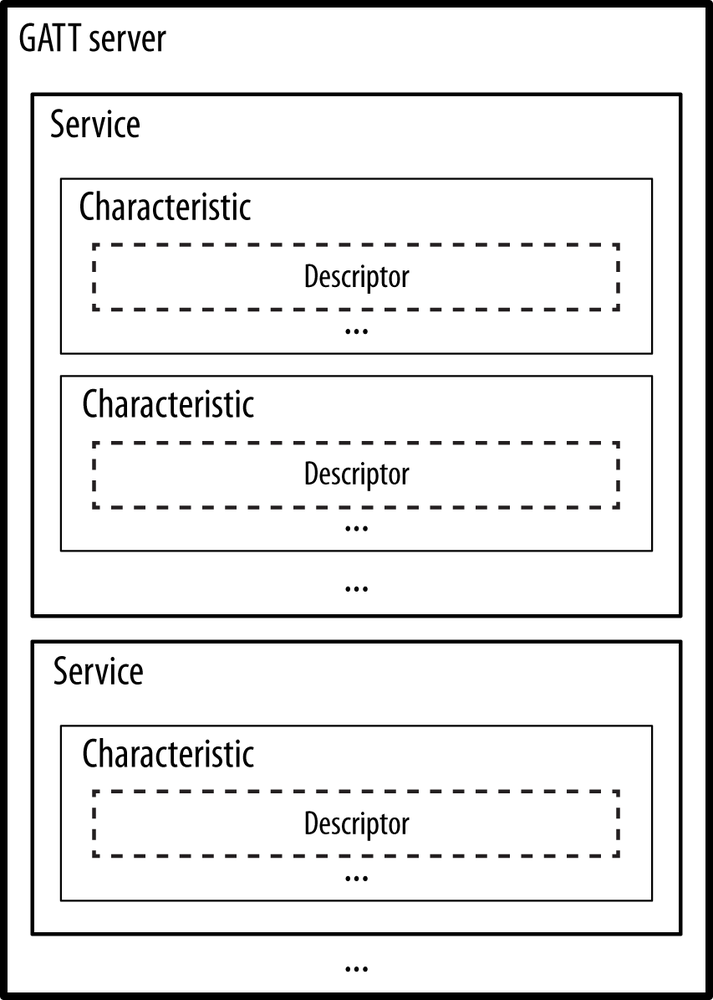
\includegraphics[width=8 cm]{gatt_structure.png}
  \caption{Data structures of GATT}
\end{figure}


\section{Install bluez v5.3}
TODO

\link{http://www.bluez.org/download/} $\rightarrow$ bluez-5.27.tar.xz

bluez 5.27 : 
\begin{lstlisting}[language=bash]
$ sudo apt-get install libdbus-1-dev libudev-dev libical-dev
Error : "checking systemd system unit dir... configure: error: systemd system unit directory is required"
\end{lstlisting}
\link{http://askubuntu.com/questions/343663/ubuntu-13-04-and-bluez-5-8-configure-error-systemd-system-unit-directory-is-re}
\begin{lstlisting}[language=bash]
$ ./configure --prefix=/usr --mandir=/usr/share/man --sysconfdir=/etc --localstatedir=/var --enable-experimental --with-systemdsystemunitdir=/lib/systemd/system --with-systemduserunitdir=/usr/lib/systemd
$ make
\end{lstlisting}

\section{XPeria developer options}
For people who are facing problems in accessing developer settings here's the trick 

Go to Settings $\rightarrow$ About phone

Tap on the build number 7 times 

Enjoy developer options 

\section{Using bluetooth device}
\begin{lstlisting}[language=bash]
$ hciconfig
Devices:
  hci1  00:1A:7D:DA:71:11 
\end{lstlisting}

Resetting Bluetooth (from 
\href{http://doc.ubuntu-fr.org/bluetooth\#problemes\_connus}{ubuntu-fr.org}) :
\begin{lstlisting}[language=bash]
$ sudo rfkill unblock all
$ sudo hciconfig hci1 up

$ sudo hcitool -i hci1 lescan
D0:39:72:B7:AF:66 (unknown)
D0:39:72:B7:AF:66 Bubi
\end{lstlisting}

\section{Connecting to MiP}

\begin{lstlisting}[language=bash]
$ sudo gatttool -i hci1 -b D0:39:72:B7:AF:66 -I
> connect
\end{lstlisting}

Get handles:
\begin{lstlisting}[language=bash]
http://www.jaredwolff.com/blog/get-started-with-bluetooth-low-energy/ 
http://i-miss-erin.blogspot.fr/2010/12/gatttool-in-bluez-over-bredr.html 
\end{lstlisting}

\begin{lstlisting}[language=bash]
> primary
attr handle: 0x0011, end grp handle: 0x0014 uuid: 0000ffe5-0000-1000-8000-00805f9b34fb
Send Data Service: 0xFFE5
attr handle: 0x000c, end grp handle: 0x0010 uuid: 0000ffe0-0000-1000-8000-00805f9b34fb
Receive Data Service: 0xFFE0
\end{lstlisting}

\subsection{Discover characterstics}
\begin{lstlisting}[language=bash]
> characteristics
handle: 0x0012, char properties: 0x0c, char value handle: 0x0013, uuid: 0000ffe9-0000-1000-8000-00805f9b34fb
Send Data WRITE Characteristic: 0xFFE9
handle: 0x000d, char properties: 0x10, char value handle: 0x000e, uuid: 0000ffe4-0000-1000-8000-00805f9b34fb
Receive Data NOTIFY Characteristic: 0xFFE4
\end{lstlisting}

\subsection{Discover All Characteristic Descriptors}
\begin{lstlisting}[language=bash]
> char-desc
\end{lstlisting}

\section{Sending orders}
References:\begin{itemize}
 \item \href{https://github.com/WowWeeLabs}{WowWeeLabs}
 \item \href{https://github.com/WowWeeLabs/MiP-BLE-Protocol}{MiP-BLE-Protocol}
 \item \href{https://github.com/WowWeeLabs/MiP-BLE-Protocol/blob/master/MiP-Protocol.md}
     {Command doc}
\end{itemize}


LEDs are characteristics;
\begin{lstlisting}[language=bash]
serviceId: MIPSendDataService,   ffe5
characteristicId: MIPSendDataWrite,   ffe9
value: SetChestLED;  0x84 r g b
\end{lstlisting}

Set head LED:
\begin{lstlisting}[language=bash]
> char-write-cmd 0x0013 8A0202020201
\end{lstlisting}

Sounds:
\begin{lstlisting}[language=bash]
> char-write-cmd 0x0013 0602

> char-read-hnd 0x000e
> char-write-cmd 0x0013 780060
\end{lstlisting}

Set volume:
\begin{lstlisting}[language=bash]
char-write-cmd 13 1501
\end{lstlisting}


\section{Reading infos}
\link{https://stackoverflow.com/questions/25536695/wowwee-mip-command-over-bluetooth-in-linux-shell-with-gatttool}

\link{http://www.compulab.co.il/utilite-computer/forum/viewtopic.php?f=77\&t=1639}

Read LED:
\begin{lstlisting}[language=bash]
char-write-cmd <handle> value
> char-read-hnd 0x83
\end{lstlisting}

Get firmware version:
\begin{lstlisting}[language=bash]
> char-write-cmd 0x0013 14
Notification handle = 0x000e value: 31 34 30 45 30 33 31 36 30 32
\end{lstlisting}
Translating thanks to 
\href{http://www.rapidtables.com/convert/number/hex-to-ascii.htm}{rapidtables}:
\begin{lstlisting}[language=bash]
31 34 30 45 30 33 31 36 30 32 > 140E031602
\end{lstlisting}
Now parse each pair of consecutive chars : 
it is a int written in hex format, convert into decimal format:
\begin{lstlisting}[language=bash]
14:20 0E:14 03:03 16:22 02:02
\end{lstlisting}
The first int corresponds to the calling code: here $0x14$ for the firmware version.


Non interactive:
\link{http://www.humbug.in/2014/using-gatttool-manualnon-interactive-mode-read-ble-devices/} 

\begin{lstlisting}[language=bash]
$ sudo gatttool -i hci0 -b D0:39:72:B7:AF:66 --char-write-req -a 0x0013 -n 14 --listen
Characteristic value was written successfully
Notification handle = 0x000e value: 31 34 30 45 30 33 31 36 30 32

$ timeout .3 gatttool -i hci0 -b D0:39:72:B7:AF:66 --char-write-req -a 0x0013 -n 14 --listen
Characteristic value was written successfully
Notification handle = 0x000e value: 31 34 30 45 30 33 31 36 30 32 
\end{lstlisting}

Cut after two lines:
\link{https://superuser.com/questions/402979/kill-program-after-it-outputs-a-given-line-from-a-shell-script}

Combine both:
\begin{lstlisting}[language=bash]
timeout 1 gatttool -i hci1 -b D0:39:72:B7:AF:66 --char-write-req -a 0x0013 -n 14 --listen | grep -m 1 "value:"
\end{lstlisting}


\section{Gatttool example}
\link{https://gitorious.org/bluez/moreira-bluez-mainline/raw/0831238284de7dcf994bf9e2c350bb9acdc959e2:attrib/gatttool.c} 

\link{http://people.csail.mit.edu/albert/bluez-intro/c404.html}


\end{document}
